
\chapter{Model View Controllers}

A typical example of model synchronization occurs when a model is
visualized as a diagram. There are many software tools available that
provide access to a model via a diagram. You can create an instance
of the model by interacting with the diagram. Sometimes, the tool
also supports interacting with the model instance via other routes:
via property editors or a scripting language. Where the instance can
be modified in this way, it is important that the diagram view is
updated to be consistent. Consistency update may be automatic or may
be explicitly invoked via a refresh.

This chapter defines a modelling language, a diagram model and shows
how the two can be synchronized by modelling a mapping between them.
It turns out that the mappings conform to a small number of patterns
that can be reused to create model synchronizers.

%
\begin{figure}
\begin{center}

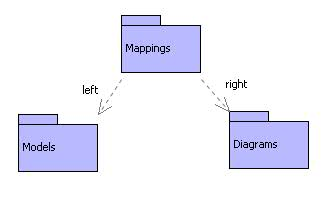
\includegraphics[width=12cm]{LanguageEngineering/MVC/Images/Sync}

\caption{\label{Mapping-Overview}Overview}

\end{center}
\end{figure}


Figure \ref{Mapping-Overview} provides an overview of the synchronization
architecture for the example. The left-hand package defines a simple
data modelling language consisting of the usualy components: packages;
classes; attributes and inheritance. The right-hand package defines
a simple model for diagrams including: diagrams; nodes; edges and
display elements. A diagram display element has a position and may
be either a box (container of display elements) or a text string.

The package in the centre contains a definition of mappings that are
used to synchronize models and diagrams. The idea is that a mapping
connects instances from the left with their corresponding instances
on the right such that when a change occurs on one side, the change
can be reflected in the corresponding element on the other side.

%
\begin{figure}
\begin{center}

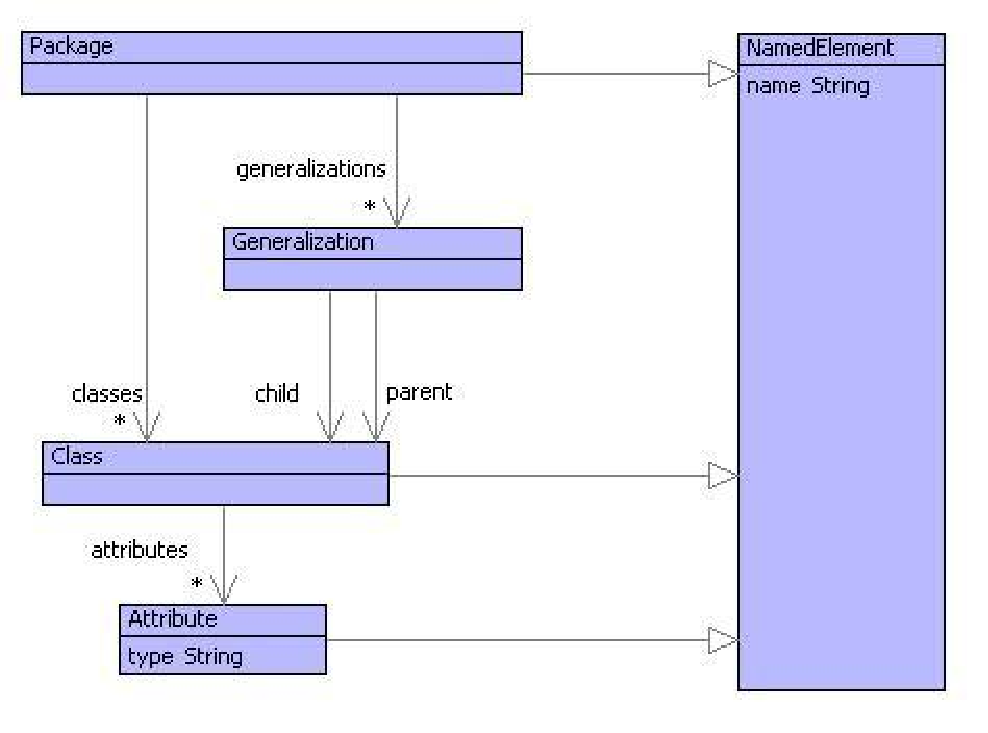
\includegraphics[width=12cm]{LanguageEngineering/MVC/Images/Models}

\caption{\label{Data-Models}Data Models}

\end{center}
\end{figure}



\section{Model-Diagram Synchronization}

Here's an example. Support there is a class named C in a package.
Then there should be a diagram with a node for C. The node for C contains
a box which in turn contains a text item whose text is the string
{}``C''. Mappings are used to:

\begin{itemize}
\item connect the package to the diagram
\item connect the class to the node
\item connect the class name to the text item
\end{itemize}
Suppose that the name of C is changed on the diagram by editing the
text item. The change is propagated to the mapping between the class
name and the text item. Since the text item has changed, the class
is updated to be consistent. Alternatively, if the class name is changed
then the mapping allows the change to be propagated to the text item.

%
\begin{figure}
\begin{center}

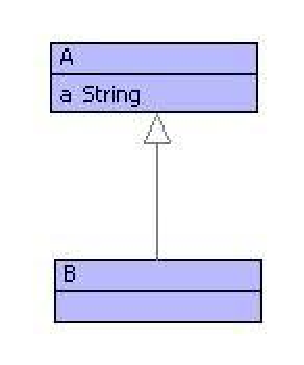
\includegraphics[width=12cm]{LanguageEngineering/MVC/Images/Example}

\caption{Example\label{Example-Model}}

\end{center}
\end{figure}


Notice that in both the scenarios given above, it was not necessary
for the model element to know about the diagram element and vice versa.
This is an important issue: when model instances are synchronized,
the machinery must ensure a separation of concerns. There is no reason
why the model should know about the diagram -- to do so would compromise
reusability of the model. Similarly, if the diagram elements are directly
associated with the model elements then this makes it difficult to
use the diagram model in a variety of circumstances (domain specific
languages for example).


\section{Models}

%
\begin{figure}
\begin{center}

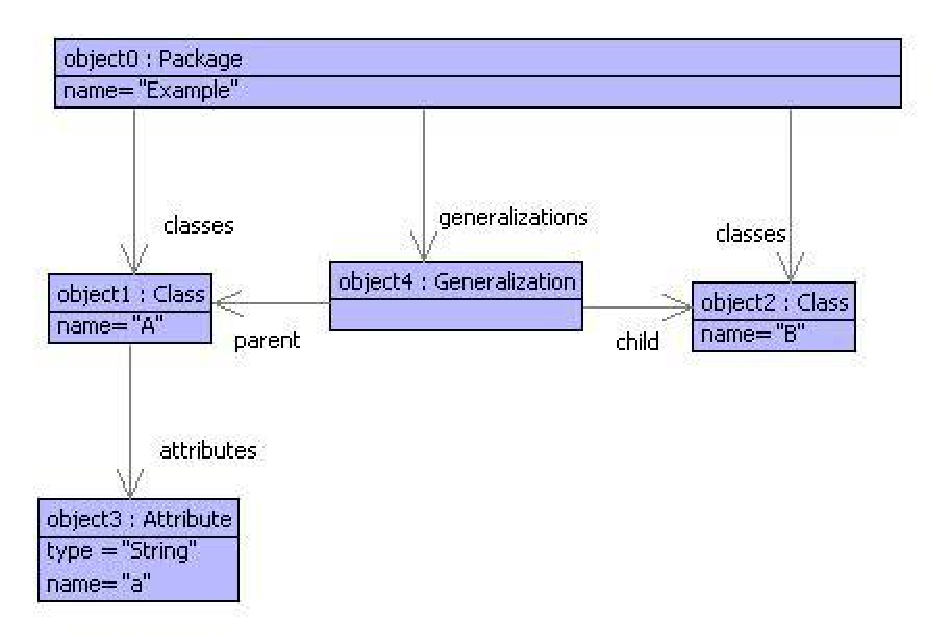
\includegraphics[width=12cm]{LanguageEngineering/MVC/Images/ModelSnapshot}

\caption{Model Snapshot\label{Model-Snapshot}}

\end{center}
\end{figure}


Figure \ref{Data-Models} shows a simple data model consisting of
packages, classes, attributes and generalizations. This model is representative
of many data modelling notations. 

Figure \ref{Example-Model} shows an example model as it would be
seen in a diagram editor. The snapshot shown in figure \ref{Model-Snapshot}
shows the same model as an instance of figure \ref{Data-Models}.


\section{Diagrams}

Diagrams contain nodes with edges between them. Each node has a position
on the diagram and contains a collection of displays. A display has
a co-ordinate that is relative to its container; it may be a text
item or a box (bordered container of display elements). The model
for diagrams is shown in figure \ref{fig:Diagrams}.

%
\begin{figure}
\begin{center}

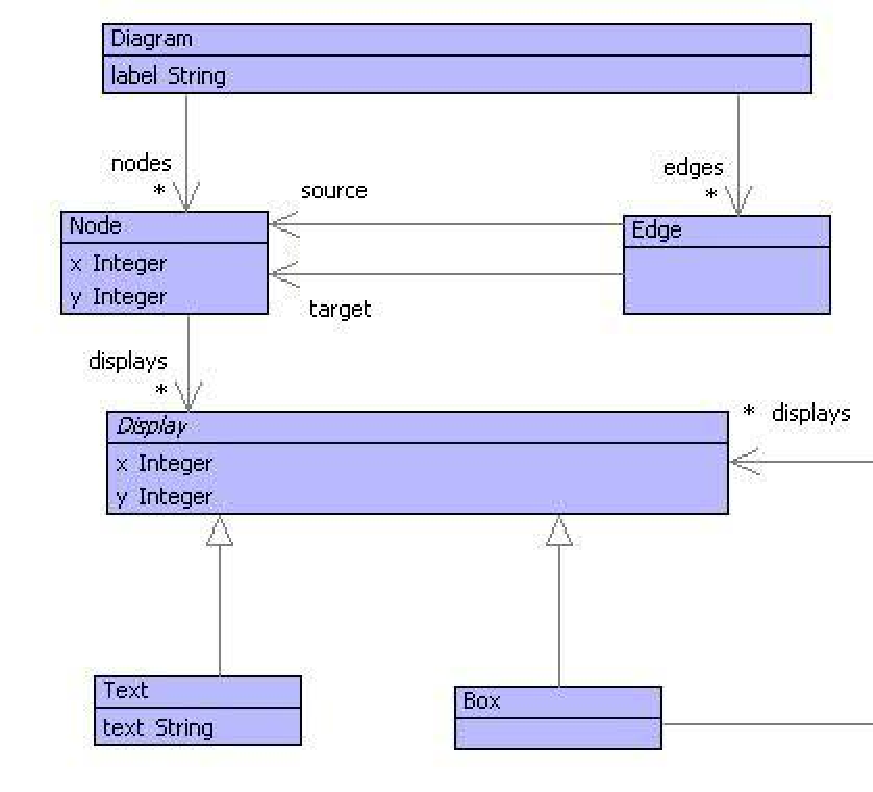
\includegraphics[width=12cm]{LanguageEngineering/MVC/Images/Diagrams}

\caption{\label{fig:Diagrams}Diagrams}

\end{center}
\end{figure}


%
\begin{figure}
\begin{center}

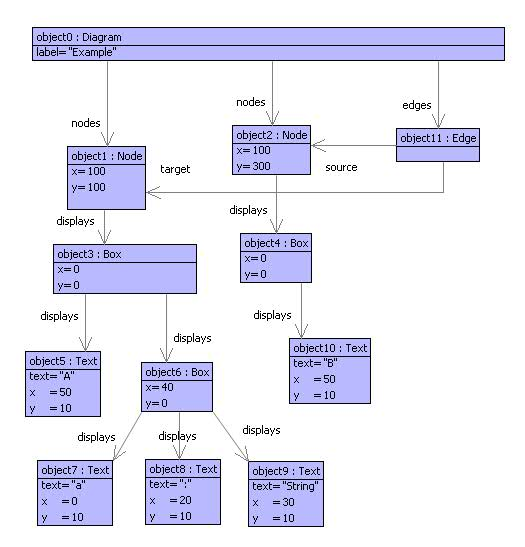
\includegraphics[width=12cm]{LanguageEngineering/MVC/Images/DiagramSnapshot}

\caption{Diagram Snapshot\label{fig:Diagram-Snapshot}}

\end{center}
\end{figure}


The diagram of the model shown in figure \ref{Example-Model} is shown
in figure \ref{fig:Diagram-Snapshot}. A diagram has a label that
is intended to be the same as the name of the corresponding package.
Each class is shown as a node and generalizations are shown as edges
between class nodes. A class is drawn as a box, with the name as a
text item at the top followed by attribute boxes. Each attribute box
contains text items for the name, {}``:'' and the type of the attribute.
Note that in the example, the positions of the nodes and displays
are illustrative.

Diagrams know nothing about classes, attributes and generalizations.
This is as it should be since we could choose to use the diagram model
to display a variety of information including class-models, snapshot-models,
CPM networks and decision trees.


\section{Mappings}

%
\begin{figure}
\begin{center}

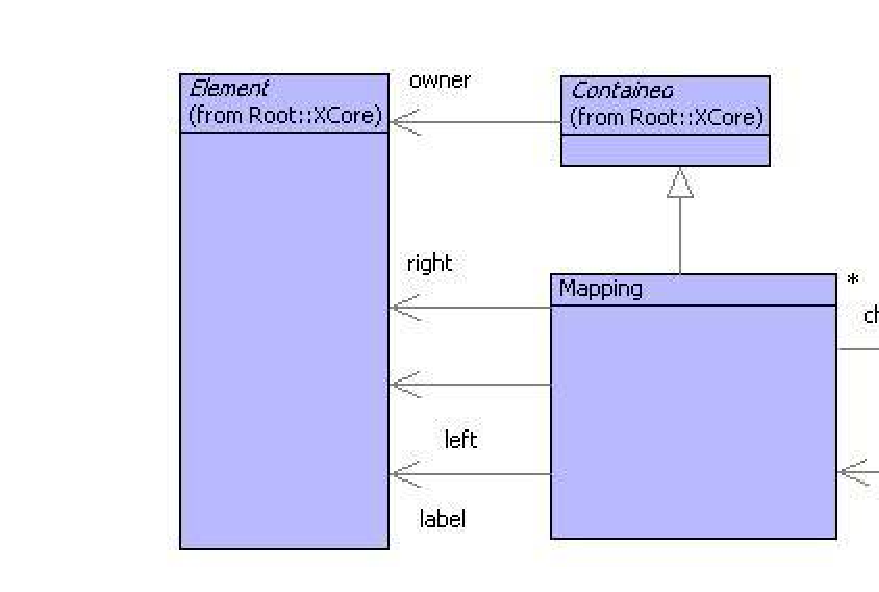
\includegraphics[width=12cm]{LanguageEngineering/MVC/Images/Mappings}

\caption{\label{fig:Mappings}Mappings}

\end{center}
\end{figure}


Figure \ref{fig:Mappings} shows a model of mappings that can be used
to synchronize a class-model with a diagram. A mapping is a tree structure
that link elements from a left-hand model with elements from a right-hand
model. Each mapping has a label that can be used to distinguish between
different mappings between the same left and right elements.

Mappings sit between the left and right-hand elements in order to
record the fact that they should be the same in some sense. As such,
a mapping can have intimate knowledge of the left and right-hand model
structures. In the case of a class-model and a diagram, mappings can
be expected to know that a class has a name and the related diagram
node has a text item that is used to display the class name. Neither
the class-model or the diagram model know anything about each other,
so there is a clear division of concerns: cross-model information
is limited to the mapping.

Mappings can be used to relate any elements from the left and right-hand
models and a mapping is is a tree structured thing (made up of \textit{maplets}).
It is up to us as modellers to decide how to structure and use the
mapping. Each mapping has children that are other mapping components.
The idea is that if the left and right elements are composed of children
then the mapping will have maplets that appropriately relate those
children. For example, a package may be related to a diagram via a
mapping composed of maplets that relate the package's classes with
the diagram's nodes.

Mappings simply record the associations between left and right-hand
elements. There is no requirement for mappings to be used in any particular
way. However, it turns out that there are useful patterns of mapping
usage, both in terms of how they relate models that are themselves
structured using standard patterns.

%
\begin{figure}
\begin{center}

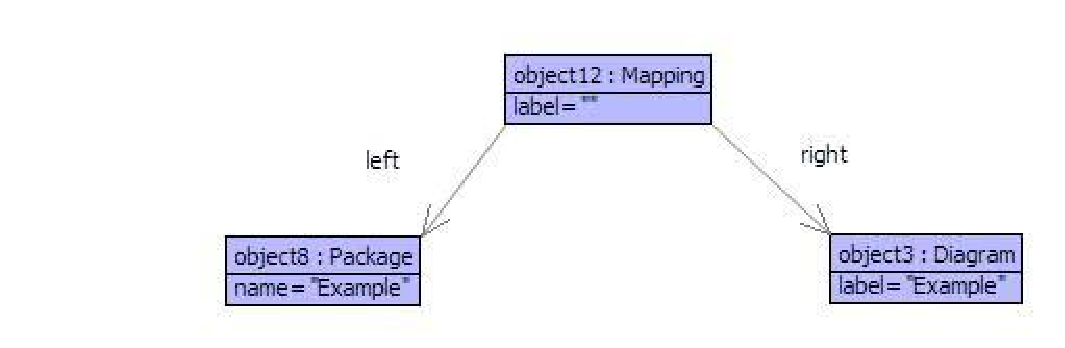
\includegraphics[width=12cm]{LanguageEngineering/MVC/Images/MappingSnapshot1}

\caption{\label{fig:A-Package-Mapping}A Package Mapping}
\end{center}
\end{figure}


Figure \ref{fig:A-Package-Mapping} shows how a package and a diagam
are associated using mappings. This is a root mapping and is responsible
for synchronizing the package with all its components against the
diagram with all its components. The mapping object12 is individually
responsible for keeping the name of the package synchronized with
the diagram label; it devolves responsibility for the class and generalization
synchronization to its child maplets.

%
\begin{figure}
\begin{center}

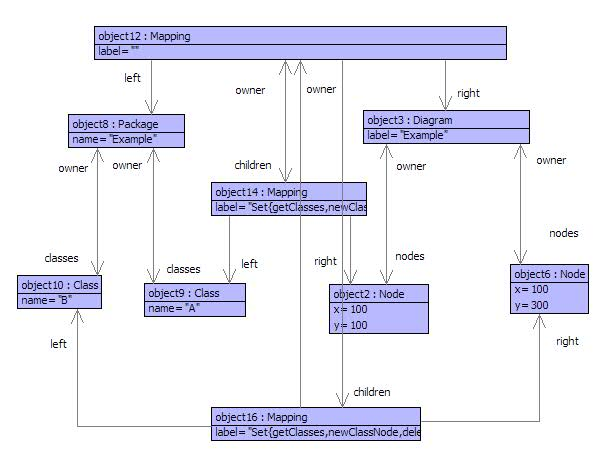
\includegraphics[width=12cm]{LanguageEngineering/MVC/Images/MappingSnapshot2}

\caption{\label{fig:Class-Mappings}Class Mappings}

\end{center}
\end{figure}


Figure \ref{fig:Class-Mappings} shows the child maplets of the root
package/diagram mapping. The root mapping has two children:; object14
and object16 that are responsible for associating classes A and B
with their corresponding diagram nodes. In each case the maplets have
labels (the detail of which is not shown) that identify them as being
\textit{class-associating} mappings.

It is worth considering how this mapping migh be used as part of a
tool. Suppose that the name of the package (object8) is modified,
to X. The resulting event causes a synchronization to occur (or the
user manually causes a synchronization to occur) which in turn asks
the mapping (object12) to synchronize its left and right elements.
At this stage, the name at object8 is X whereas the label at objct3
is Example. The mapping object12 detects this inconsistency and modifies
the label (causing a chage in the GUI). The story would be much the
same if the label was changed causing the packag name to be modified.

Now consider what happens if we add a class node to the diagram. Suppose
that objects 6, 16 and 10 have yet to be added (i.e. the model contains
only class A). The user adds a node to the diagram (object6) and the
synchronization is started, as before, at object12. 

Part of the synchronization task of object12 is to ensure that, if
the diagram has changed, every node has a corresponding class. The
mapping object12 can do this because it has access to (and knowledge
of) both packages and diagrams. When this check is performed, object12
detects that there is a node (object6) for which there is no child
maplet. Therefore, the model and diagram are inconsistent. The remedy
is to create a class (object10) and associate it via a new maplet
object16 with the diagam node. The story is much the same if a class
is added to the model: a new node is added to the diagram and a maplet
to the root mapping.

\section{Mapping Patterns}

Mappings are used to link left-hand instances to rght-hand instances
and mappings are structured into trees of maplets. So far, synchronization
has been described in rather hand-wavy terms. This is because, in
general, many different synchronization strategies and implementations
are possible ranging from those that are implemented by hand (and
guided by the mappings) to those that are fully automated.

In many circumstances, it is possible to define mapping patterns such
that mappings can be applied to instances of left and right models
in chunks. Moreover, the pattern chunks can be made to be self manging
in terms of synchronization. The next couple of sections show how
an analysis of the model-diagram example leads to patterns and then
shows how the patterns can be defined in XMF. The following section
then gives the full implementation of the model diagram application
in terms of the patterns.


\section{Equality Pattern}

Consider classes and attributes. They have a feature in common: they
both have names. Consider class diagrams and the rendering of classes
and attributes. They are each rendered as text items in boxes such
that the synchronization ties up the name with the string in the text
item.

Class and attribute name synchronization is an example of and \textit{equality
pattern}. Where a left-hand item (the name) is defined to be equal
to a right-hand item (the string). The difference between the two
examples, occurs in terms of how the name/string is accessed, updated
and created.

Suppose that an equality synchronization pattern is defined. What
are its different modes of operation:

\begin{enumerate}
\item If a left-hand instance exists but a right-hand instance does not
then the maping is being used to genrate the right from the left.
It must be possible to creat a new instance of the appopriate right-hand
element and link it to the left with a maplet.
\item If a left-hand instance changes then we must be able to update the
right-hand instance.
\item If a right-hand instance exists, but a left-hand instance does not
then proceed as for 1 (right to left).
\item If a right-hand instance chages then proceed as for 2 (right to left).
\end{enumerate}
There are clearly two major modes (left, right) each of which has
minor modes (in-sync, update, generate). Assuming that it is always
possible to tell which side has changed, the two major modes can be
defined separately. The following XMF operation definition gives the
laft-major mode definition for the equality pattern:

\begin{lstlisting}
@Operation syncEqualLeft(lab,getLeft,setRight,newRight,mapping)
(1)  let left = mapping.left();
         right = mapping.right()
(2)  in @Find(child,mapping.children())
(3)       when child.label() = lab
(4)       do if getLeft(left) <> child.left()
             then
(5)            child.setLeft(getLeft(left));
               child.setRight(getLeft(left));
               setRight(right,getLeft(left))
          end
         else
(6)        let new = newRight(right,getLeft(left)) then
(7)            child = Mapping(lab,getLeft(left),new)
(8)        in mapping.addToChildren(child)
           end
        end
    end
  end
\end{lstlisting}The operation syncEqualLeft takes 5 arguments: a label used to mark
the equality maplet; an accessor for the left-hand element; an updater
for the right-hand element; a creator for the right-hand element;
and a mapping. The mapping associates two elements that have sub-components
related by equality. For example, the mapping may associate a package
and a diagram such that the name and label are syncronized. For example,
the mapping may associate a class and a node such that the class-name
and the string in a text item are synchronized.

Line (1) extracts the left and right elements from the mapping. Lines
(2-3) select a maplet linking the synchronized elements. If this exists
then a check is made at (4) to see if the leftt-hand element has changed.
If it has changed then the element will be out of sync with the maplet
and lines (5-) update the appropriate components thereby synchronizing.

Line (6) occurs when the maplet for the synchronized elements dos
not exist. This occurs when the right-hand element is being generated
from the left. In this case, a new right-hand element is constructed
(6). Imagine class-names being synchronized with text items: the arguments
in (6) are the node and the class-name.

Line (7) creates a new maplet (assumed synchronized) and (8) adds
the maplet to the parent mapping.


\section{Containment Pattern}

Consider packages and classes (similarly classes and attributes) compared
with diagrams and nodes (similarly nodes and contained boxes). In
both cases one element contains a collection of sub-elements: packages
contain classes; diagrams contain nodes. Synchronization of such elements
can be captured as a containment pattern with the following modes:

\begin{enumerate}
\item Addition of a new left-hand instance (e.g. a class) causes addition
of a corresponding right-hand instance (e.g. a node).
\item Deletion of a left-hand instance causes deletion of the corresponding
right-hand instance.
\item Addition of a right-hand instance (as for 1 but right to left).
\item Deletion of a right-hand instance (as for 2 but right-to-left).
\end{enumerate}
The pattern can be applied to mny different types of containment structure.
The differences occur in terms of access to, creation of and deletion
of the contained elements. Also, as for equality, there are two modes
depending on whether the left hand element has chaged or the right.
The left-hand mode is defined by the following XMF operation:

\begin{lstlisting}
@Operation syncSetsLeft(lab,getLeft,newRight,deleteRight,mapping,subSync)
(1) let left = mapping.left();
        right = mapping.right()
(2) in @For x in getLeft(left) do
(3)      @Find(child,mapping.children())
(4)        when child.left() = x
(5)        do subSync(child)
           else
(6)          let y = newRight(mapping,x,right) then
(7)              child = Mapping(lab,x,y)
(8)          in mapping.addToChildren(child);
(9)             subSync(child)
             end
         end
       end;
(a)    @For child in mapping.children() 
(b)      when child.label() = lab 
(c)      do @Find(x,getLeft(left))
(d)           when child.left() = x
              else
(e)             mapping.deleteFromChildren(child);
(f)             deleteRight(right,child.right())
            end
       end
    end
  end
\end{lstlisting}The operation syncSetsLeft expects 6 arguments:; a label used to tag
maplets; an accessor for components of the left element; a constructor
for new right-hand elements; an operation that deletes right-hand
elements, a mapping and an element synchronizer.

Line (1) extracts the left and right-hand elements. Each sub-component
x is extracted at (2) and handled in turn. A maplet that associates
x is extracted at (3-4). If the maplet child exists then the synchronizer
is applied to it.

Otherwise (6) creates a new right-hand element, (7) creates a new
maplet, (8) adds the maplet to the parent mapping and (9) applies
the synchronizer.

Lines (a-f) check whether any children have been deleted from the
left-hand element. At (e) a maplet exists for which there is no longer
a sub-component x. In this case (e) removes the maplet and (f) deletes
the right-hand element.


\section{Model-Diagam Implementation}

The model-diagram synchronizer can now be implemented in terms of
the patterns defined in the previous sections. A synchronizer is an
operation that accepts a mapping and synchronizes the left and right-hand
elements. The implementation of the synchronizer that is used when
a model eleent changes is shown below:

\begin{small}
\begin{lstlisting}
@Operation syncPackage(mapping)
  syncEqualLeft("name",
    getName,
    setLabel,
    newLabel,
    mapping);
  syncSetsLeft("classes",
    getClasses,
    newClassNode,
    deleteClassNode,
    mapping,
    syncClass);
  syncSetsLeft("inherits",
    getGens,
    newGenEdge,
    deleteGenEdge,
    mapping,
    emptyMap)
end
  
@Operation syncClass(mapping)
  syncEqualLeft("name",
    getName,
    setClassNodeName,
    newClassNodeName,
    mapping);
  syncSetsLeft("atts",
    getAtts,
    newAttBox,
    deleteAttBox,
    mapping,
    syncAttribute)
end
  
@Operation syncAttribute(mapping)
  syncEqualLeft("att",
    getNameAndType,
    setNameAndType,
    newNameAndType,
    mapping)
end
\end{lstlisting}
\end{small}

The operation syncPackage causes changes in the package name to update
the diagram label, changes in the package classes to update the nodes
on the diagram, and chages in the generalization links to cause corresponding
changes in the diagram. Each class is synchronized using syncClass.

The operation syncClass causes chages in the class name to update
the text in the class node name box, and changes to the class attributes
to cause corresponding changes to the boxes on the diagram.


\section{A Simple Database Synchronizer}

The following shows how the patterns can be used to synchronise packages
and classes with database tables. A table is represented simply as
a sequence of records. Each record is just a sequence of field values: 

\begin{lstlisting}
Root::Packages := Seq{};

Root::ClassSets := Seq{};

Root::Classes := Seq{};
  
context Root
  @Operation deleteClass(table,id)
    Root::ClassSets := table->reject(r | r->head = id)
  end
  
context Root
  @Operation setPackageName(id,name)
    @Find(package,Packages)
      when package->head = id
      do Root::Packages := 
           Packages->excluding(package)
                   ->including(Seq{id,name,package->at(2)});
         name
    end
  end
  
context Root
  @Operation newClassRecord(map,class,pid)  
    @Find(package,Packages)
      when package->head = pid
      do let C = ClassSets->select(r | r->head = package->at(2));
             cid = "C" + Classes->size
         in Root::ClassSets := 
              ClassSets->including(Seq{package->at(2),cid});
            Root::Classes := 
              Classes->including(Seq{cid,class.name()});
            cid
         end
    end
  end
  
context Root
  @Operation deleteClassRecord(pid,cid)
    @Find(package,Packages)
      when package->head = pid
      do let Cid = package->at(2)
         in @Find(C,ClassSets)
              when C->head = Cid and C->at(1) = cid
              do Root::ClassSets := ClassSets->excluding(C);
                 Root::Classes := Classes->reject(r | r->head = cid)
            end
         end
    end
  end
  
context Root
  @Operation syncPackageTable(mapping)
    syncEqualLeft(getName,setPackageName,setPackageName,mapping);
    syncSetsLeft(getClasses,newClassRecord,deleteClassRecord,mapping,emptyMap)
  end
\end{lstlisting}
